\section{Aufgabenstellung}
\label{chap:basics}
Bei der Projektaufgabe `Damespiel' geht es grundsätzlich darum eine Art künstliche Intelligenz --- basierend auf den vorgstellten Algorithmen des Moduls --- zu entwickeln, welche fähig ist eine Urform des Damespiels autonom und möglichst optimal zu spielen.

\subsection{Spielbrett}
\label{sec:board}
Als Spielbrett dient dabei eine modifizierte Version des klassichen Schachbretts --- ein Spielbrett mit abwechselnd schwarzen und weissen Feldern der Grösse 5 auf 5. Es existeren zwei Parteien, eine Partei mit schwarzen und eine Partei mit weissen Steinen.Jede Partei erhält dabei 12 Steine. Im Gegensatz zum klassischen Damespiel, wo nur die schwarzen Felder mit Steinen besetzt werden, werden alle Felder mit Steinen besetzt. Die Verteilung ist so, dass die Steine der Spieler auf je eine Hälfte aufgeteilt werden. Die mittlere Reihe enthält dann jeweils zwei Steine pro Partei, das mittlere Feld bleibt leer.

\begin{figure}[h]
\centering
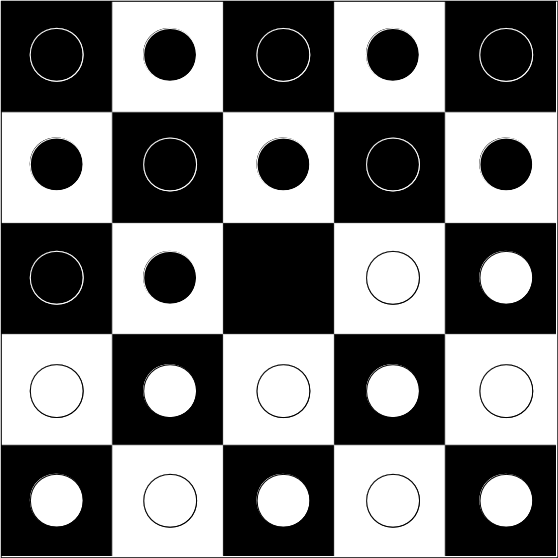
\includegraphics[width=200px]{images/checkers_board.png}
\caption[width=100px]{Darstellung Spielbrett mit Initialstellung\protect\footnotemark}
\label{fig:checkersBoardInitial}
\end{figure}
\footnotetext{Eigene Darstellung mittels Libre Office Impress und Gimp}

\subsection{Regeln}
\label{sec:rules}
Im Spiel wird abwecheslungsweise gespielt und pro Zug darf maximal ein Stein gezogen werden. Grundsätzlich sind alle Bewegungsrichtungen möglich --- sofern das angestrebte Feld frei ist. Ist ein Feld von einem gegenrischen Stein blockiert, das direkt hinter dem Stein liegende Feld aber frei, so darf der gegnerische übersprungen werden. Dabei wird der übersprungene Stein vom Feld entfernt. Im Gegensatz zur klassischen Variante des Damespiels gibt es in der hier beschriebenen Variante keine Ketten. Dies heisst, dass ein Spieler mit einem Stein gleich mehrere gegnerische Steine nacheinander überpspringen kann. Dabei gilt die zuvor beschriebene Regel.

\begin{minipage}[t]{0.4\textwidth}
    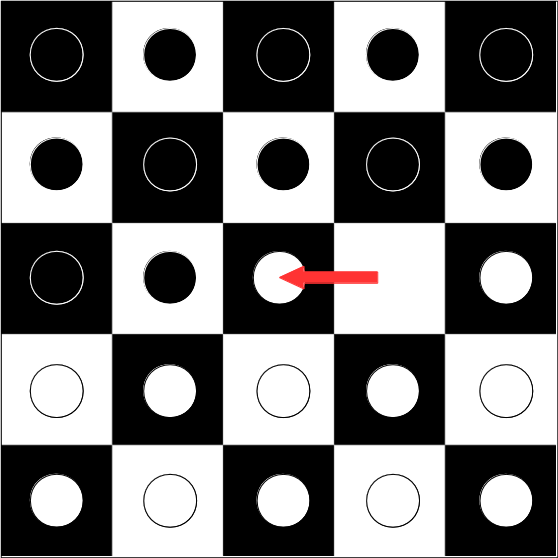
\includegraphics[width=\textwidth]{images/checkers_rule_01.png}
    \captionof{figure}{Seitwärtsbewegung eines weissen Steins\protect\footnotemark}
\label{fig:checkersRule01}
\end{minipage}
\footnotetext{Eigene Darstellung mittels Libre Office Impress und Gimp}
\begin{minipage}[t]{0.4\textwidth}
    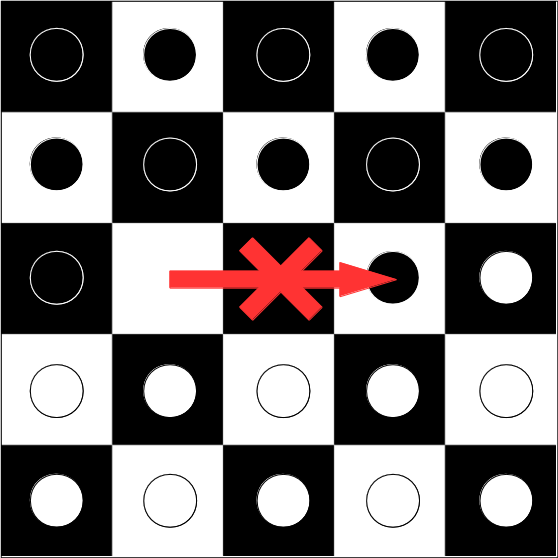
\includegraphics[width=\textwidth]{images/checkers_rule_02.png}
    \captionof{figure}{Ein schwarzer Stein übersrpingt einen weissen Stein\protect\footnotemark}
\label{fig:checkersRule02}
\end{minipage}
\footnotetext{Eigene Darstellung mittels Libre Office Impress und Gimp}
